\chapter{Locking}
\label{CH:LOCK}

Most kernels, including xv6, interleave the execution
of multiple activities.
One source of interleaving is multiprocessor hardware:
computers with
multiple CPUs executing independently, such as xv6's RISC-V.
These multiple CPUs share physical RAM,
and xv6 exploits the sharing to maintain
data structures that all CPUs read and write.
This sharing raises the possibility of
one CPU reading a data structure while another
CPU is mid-way through updating it, or even
multiple CPUs updating the same data simultaneously;
without careful design such parallel access is likely
to yield incorrect results or a broken data structure.
Even on a uniprocessor, the kernel may switch the CPU among
a number of threads, causing their execution to be interleaved.
Finally, a device interrupt handler that modifies
the same data as some interruptible code could damage
the data if the interrupt occurs at just the wrong time.
The word 
\indextext{concurrency}
refers to situations in which
multiple instruction streams are interleaved,
due to multiprocessor parallelism,
thread switching, or interrupts.

Kernels are full of concurrently-accessed data. For example, two CPUs
could simultaneously call {\tt kalloc}, thereby concurrently
popping from the head of the free list. Kernel designers like to allow
for lots of concurrency, since it can yield increased performance
though parallelism, and increased responsiveness. But, as a result,
kernel designers spend a lot of effort convincing themselves of
correctness despite such concurrency. There are many ways to arrive at
correct code, some easier to reason about than others. Strategies
aimed at correctness under concurrency, and abstractions that support
them, are called \indextext{concurrency control} techniques. Xv6 uses
a number of concurrency control techniques, depending on the
situation; many more are possible. This chapter focuses on a widely
used technique: the \indextext{lock}.

A lock provides mutual exclusion, ensuring that only one CPU at a time can hold
the lock. If the programmer associates a lock with each shared data item,
and the code always holds the associated lock when using an item,
then the item will be used by only one CPU at a time.
In this situation, we say that the lock protects the data item.

The rest of this chapter explains why xv6 needs locks, how xv6
implements them, and how it uses them.


% The following is most relevant to lock-free code:
% 
% A key observation will be that if you look at some code in
% xv6, you must ask yourself if concurrent code could change
% the intended behavior of the code by modifying data (or hardware resources)
% it depends on.
% You must keep in mind that the compiler may turn a
% single C statement into several machine instructions,
% and that those instructions may execute in a way that is
% interleaved with instructions executing on other CPUs.
% That is, you cannot assume that lines of C code
% on the page are executed atomically.
% Concurrency makes reasoning about correctness difficult.

%% 
\section{Race conditions}
%% 

As an example of why we need locks,
consider a linked list accessible from any
CPU on a multiprocessor.
The list supports push and pop operations, which
may be called concurrently.
Xv6's memory allocator works in much this way;
\lstinline{kalloc()}
\lineref{kernel/kalloc.c:/^kalloc/}
pops a page of memory from a list of free pages,
and
\lstinline{kfree()}
\lineref{kernel/kalloc.c:/^kfree/}
pushes a page onto the free list.

If there were no
concurrent requests, you might implement a list
\lstinline{push}
operation as follows:
\begin{lstlisting}[numbers=left,firstnumber=1]
    struct element {
      int data;
      struct element *next;
    };
    
    struct element *list = 0;
    
    void
    push(int data)
    {
      struct element *l;
   
      l = malloc(sizeof *l);
      l->data = data;
      l->next = list; (*@\label{line:next}@*)
      list = l;  (*@\label{line:list}@*)
   }
\end{lstlisting}

\begin{figure}[t]
\center
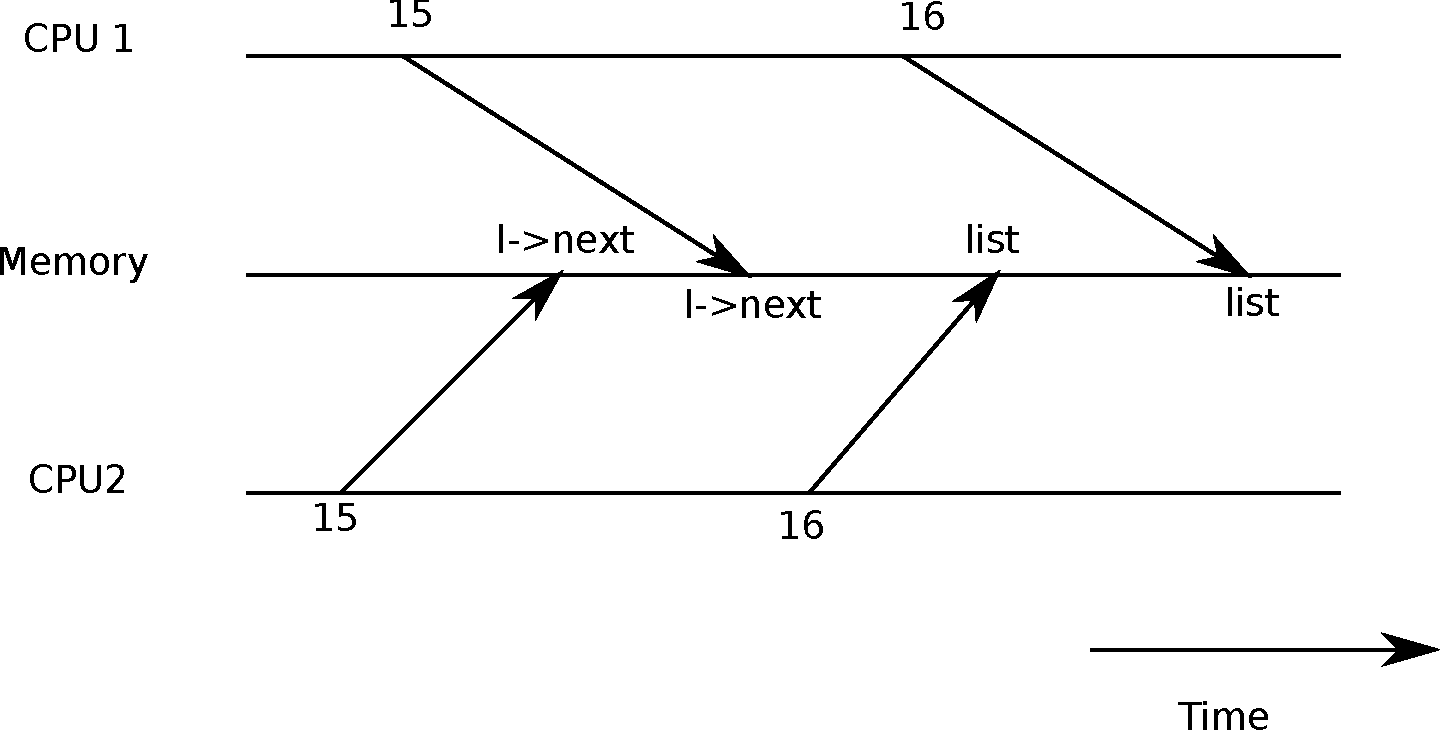
\includegraphics[scale=0.5]{fig/race.pdf}
\caption{Example race}
\label{fig:race}
\end{figure}
This implementation is correct if executed in isolation.
However, the code is not correct if more than one
copy executes concurrently.
If two CPUs execute
\lstinline{push}
at the same time,
both might execute line~\ref{line:next},
before either executes line~\ref{line:list},  (see 
Figure~\ref{fig:race}).
There would then be two
list elements with
\lstinline{next}
set to the former value of
\lstinline{list}.
When the two assignments to
\lstinline{list}
happen at line ~\ref{line:list},
the second one will overwrite the first;
the element involved in the first assignment
will be lost.

The lost update at line~\ref{line:list} is an example of a
\indextext{race condition}.
A race condition is a situation in which a memory location is accessed
concurrently, and at least one access is a write.
A race is often a sign of a bug, either a lost update
(if the accesses are writes) or a read of
an incompletely-updated data structure.
The outcome of a race depends on
the exact timing of the two CPUs involved and
how their memory operations are ordered by the memory system,
which can make race-induced errors difficult to reproduce
and debug.
For example, adding print statements while debugging
\lstinline{push}
might change the timing of the execution enough
to make the race disappear.

The usual way to avoid races is to use a lock.
Locks ensure
\indextext{mutual exclusion},
so that only one CPU at a time can execute 
the sensitive lines of
\lstinline{push};
this makes the scenario above impossible.
The correctly locked version of the above code
adds just a few lines (highlighted in yellow):
\begin{lstlisting}[numbers=left,firstnumber=6]
   struct element *list = 0;
   (*@\hl{struct lock listlock;}@*)
    	
   void
   push(int data)
   {
     struct element *l;
     l = malloc(sizeof *l); (*@\label{line:malloc}@*)
     l->data = data;
   
     (*@\hl{acquire(\&listlock);} @*)
     l->next = list;     (*@\label{line:next1}@*)
     list = l;           (*@\label{line:list1}@*)
     (*@\hl{release(\&listlock)}; @*)
   }
\end{lstlisting}
The sequence of instructions between
\lstinline{acquire}
and
\lstinline{release}
is often called a
\indextext{critical section}.
The lock is typically said to be protecting
\lstinline{list}.

When we say that a lock protects data, we really mean
that the lock protects some collection of invariants
that apply to the data.
Invariants are properties of data structures that
are maintained across operations.
Typically, an operation's correct behavior depends
on the invariants being true when the operation
begins.  The operation may temporarily violate
the invariants but must reestablish them before
finishing.
For example, in the linked list case, the invariant is that
\lstinline{list}
points at the first element in the list
and that each element's
\lstinline{next}
field points at the next element.
The implementation of
\lstinline{push}
violates this invariant temporarily: in line~\ref{line:next1},
\lstinline{l}
points
to the next list element, but
\lstinline{list}
does not point at
\lstinline{l}
yet (reestablished at line~\ref{line:list1}).
The race condition we examined above
happened because a second CPU executed
code that depended on the list invariants
while they were (temporarily) violated.
Proper use of a lock ensures that only one CPU at a time
can operate on the data structure in the critical section, so that
no CPU will execute a data structure operation when the 
data structure's invariants do not hold.

You can think of a lock as
\indextext{serializing}
concurrent critical sections so that they run one at a time,
and thus preserve invariants (assuming the critical sections
are correct in isolation).
You can also think of critical sections guarded by the same lock as being
atomic with respect to each other,
so that each sees only the complete set of
changes from earlier critical sections, and never sees
partially-completed updates.
We say that multiple processes \indextext{conflict} if they
want the same lock at the same time, or that the
lock experiences \indextext{contention}.

Note that it would be correct to move
\lstinline{acquire}
earlier in
\lstinline{push.}
For example, it is fine to move the call to
\lstinline{acquire}
up to before line~\ref{line:malloc}.
This may reduce parallelism because then the calls
to
\lstinline{malloc}
are also serialized.
The section ``Using locks'' below provides some guidelines for where to insert
\lstinline{acquire}
and
\lstinline{release}
invocations.
%% 
\section{Code: Locks}
%% 
Xv6 has two types of locks: spinlocks and sleep-locks.
We'll start with spinlocks.
Xv6 represents a spinlock as a
\indexcode{struct spinlock}
\lineref{kernel/spinlock.h:/struct.spinlock/}.
The important field in the structure is
\lstinline{locked},
a word that is zero when the lock is available
and non-zero when it is held.
Logically, xv6 should acquire a lock by executing code like
\begin{lstlisting}[numbers=left,firstnumber=21]
   void
   acquire(struct spinlock *lk) // does not work!
   {
     for(;;) {
       if(lk->locked == 0) {  (*@\label{line:test}@*)
         lk->locked = 1;      (*@\label{line:assign}@*)
         break;
       }
     }
   }
\end{lstlisting}
Unfortunately, this implementation does not
guarantee mutual exclusion on a multiprocessor.
It could happen that two CPUs simultaneously
reach line~\ref{line:test}, see that 
\lstinline{lk->locked}
is zero, and then both grab the lock by executing line~\ref{line:assign}.
At this point, two different CPUs hold the lock,
which violates the mutual exclusion property.
What we need is a way to
make lines \ref{line:test} and \ref{line:assign} execute as an
\indextext{atomic}
(i.e., indivisible) step.

Because locks are widely used,
multi-core processors usually provide instructions that
implement an atomic version of
lines~\ref{line:test} and \ref{line:assign}.
On the RISC-V this instruction is
\lstinline{amoswap r, a}.
\lstinline{amoswap}
reads the value at the memory address {\tt a},
writes the contents of register {\tt r} to that address,
and puts the value it read into {\tt r}.
That is, it swaps the contents of the register and the memory address.
It performs this sequence atomically, using special
hardware to prevent any
other CPU from using the memory address between the read and the write.

Xv6's 
\indexcode{acquire}
\lineref{kernel/spinlock.c:/^acquire/}
uses the portable C library call 
\lstinline{__sync_lock_test_and_set},
which boils down to the
\lstinline{amoswap}
instruction;
the return value is the old (swapped) contents of
\lstinline{lk->locked}.
The
\lstinline{acquire}
function wraps the swap in a loop, retrying (spinning) until it has
acquired the lock.
Each iteration swaps one into
\lstinline{lk->locked} 
and checks the previous value;
if the previous value is zero, then we've acquired the
lock, and the swap will have set 
\lstinline{lk->locked}
to one.
If the previous value is one, then some other CPU
holds the lock, and the fact that we atomically swapped one into
\lstinline{lk->locked}
didn't change its value.

Once the lock is acquired,
\lstinline{acquire}
records, for debugging, the CPU 
that acquired the lock.
The
\lstinline{lk->cpu}
field is protected by the lock
and must only be changed while holding the lock.

The function
\indexcode{release}
\lineref{kernel/spinlock.c:/^release/}
is the opposite of 
\lstinline{acquire}:
it clears the 
\lstinline{lk->cpu}
field
and then releases the lock.
Conceptually, the release just requires assigning zero to
\lstinline{lk->locked}.
The C standard allows compilers to implement an assignment
with multiple store instructions,
so a C assignment might be non-atomic with respect
to concurrent code.
Instead,
\lstinline{release}
uses the C library function
\lstinline{__sync_lock_release}
that performs an atomic assignment.
This function also boils down to a RISC-V
\lstinline{amoswap}
instruction.
%% 
\section{Code: Using locks}
%% 
Xv6 uses locks in many places to avoid race conditions.
To see a simple example much like
\lstinline{push}
above,
look at
\lstinline{kalloc}
\lineref{kernel/kalloc.c:/^kalloc/}
and
\lstinline{free}
\lineref{kernel/kalloc.c:/^free/}.
Try Exercises 1 and 2 to see what happens if those
functions omit the locks.
You'll likely find that it's difficult to trigger incorrect
behavior, suggesting that it's hard to reliably test whether code
is free from locking errors and races.
It is not unlikely that xv6 has some races.

A hard part about using locks is deciding how many locks
to use and which data and invariants each lock should protect.
There are a few basic principles.
First, any time a variable can be written by one CPU
at the same time that another CPU can read or write it,
a lock should be used to keep the two
operations from overlapping.
Second, remember that locks protect invariants:
if an invariant involves multiple memory locations,
typically all of them need to be protected
by a single lock to ensure the invariant is maintained.

The rules above say when locks are necessary but say nothing about when locks
are unnecessary, and it is important for efficiency not to lock too much,
because locks reduce parallelism.  If parallelism isn't important, then one
could arrange to have only a single thread and not worry about locks.  A simple
kernel can do this on a multiprocessor by having a single lock that must be
acquired on entering the kernel and released on exiting the kernel (though
system calls such as pipe reads or
\lstinline{wait}
would pose a problem).  Many uniprocessor operating systems have been converted to
run on multiprocessors using this approach, sometimes called a ``giant
kernel lock,'' but the approach sacrifices parallelism: only one
CPU can execute in the kernel at a time.  If the kernel does any heavy
computation, it would be more efficient to use a larger set of more
fine-grained locks, so that the kernel could execute on multiple CPUs
simultaneously.

As an example of coarse-grained locking, xv6's \lstinline{kalloc.c}
allocator has a single free list protected by a single lock. If
multiple processes on different CPUs try to allocate pages at the same
time, each will have to wait for its turn by spinning in {\tt
  acquire}. Spinning reduces performance, since it's not useful work.
If contention for the lock wasted a significant fraction of CPU time,
perhaps performance could be improved by changing the allocator design
to have multiple free lists, each with its own lock, to allow truly
parallel allocation.

As an example of fine-grained locking, xv6 has a separate lock for
each file, so that processes that manipulate different files can often
proceed without waiting for each others' locks. The file locking
scheme could be made even more fine-grained if one wanted to allow
processes to simultaneously write different areas of the same file.
Ultimately lock granularity decisions need to be driven by performance
measurements as well as complexity considerations.

As subsequent chapters explain each part of xv6, they
will mention examples of xv6's use of locks
to deal with concurrency.
As a preview,
Figure~\ref{fig:locktable}
lists all of the locks in xv6.

\begin{figure}[t]
\center
\begin{tabular}{ll}
{\bf Lock} & {\bf Description} \\
\midrule
bcache.lock & Protects allocation of block buffer cache entries \\
cons.lock & Serializes access to console hardware, avoids intermixed output \\
ftable.lock & Serializes allocation of a struct file in file table \\
icache.lock & Protects allocation of inode cache entries \\
vdisk\_lock & Serializes access to disk hardware and queue of DMA descriptors \\
kmem.lock & Serializes allocation of memory \\
log.lock & Serializes operations on the transaction log \\
pipe's pi->lock & Serializes operations on each pipe \\
pid\_lock & Serializes increments of next\_pid \\
proc's p->lock & Serializes changes to process's state \\
tickslock & Serializes operations on the ticks counter \\
inode's ip->lock & Serializes operations on each inode and its content \\
buf's b->lock & Serializes operations on each block buffer \\
\end{tabular}
\caption{Locks in xv6}
\label{fig:locktable}
\end{figure}

%% 
\section{Deadlock and lock ordering}
%% 
If a code path through the kernel must hold several locks at the same time, it is
important that all code paths acquire those locks in the same order.  If
they don't, there is a risk of \indextext{deadlock}.  Let's say two code paths in
xv6 need locks A and B, but code path 1 acquires locks in the order A
then B, and the other path acquires them in the order B then A.
Suppose thread T1 executes code path 1 and acquires lock A,
and thread T2 executes code path 2 and acquires lock B.
Next T1 will try to acquire lock B, and T2 will try to acquire lock A.
Both acquires will block indefinitely, because in both cases the
other thread holds the needed lock, and won't release it until
its acquire returns.
To avoid such deadlocks, all code paths must acquire
locks in the same order. The need for a global lock acquisition order
means that locks are effectively part of each function's specification: 
callers must invoke functions in a way that causes locks to be acquired
in the agreed-on order.

Xv6 has many lock-order chains of length two involving
per-process locks
(the lock in each
\lstinline{struct proc})
due to the way that
\lstinline{sleep}
works (see Chapter
\*[CH:SCHED]).
For example,
\lstinline{consoleintr}
\lineref{kernel/console.c:/^consoleintr/}
is the interrupt routine which handles typed characters.
When a newline arrives, any process that is waiting for
console input should be woken up.
To do this,
\lstinline{consoleintr}
holds
\lstinline{cons.lock}
while calling 
\indexcode{wakeup},
which acquires 
the waiting process's lock in order to wake it up.
In consequence, the global deadlock-avoiding
lock order includes the rule that
\lstinline{cons.lock}
must be acquired before any process lock.
The file system code contains xv6's longest lock chains.
For example, creating a file requires simultaneously
holding a lock on the directory, a lock on the new file's inode,
a lock on a disk block buffer, 
the disk driver's \lstinline{vdisk_lock},
and
the calling process's \lstinline{p->lock}.
To avoid deadlock, file system code always acquires locks in the order 
mentioned in the previous sentence.

Honoring a global deadlock-avoiding order can be surprisingly
difficult. Sometimes the lock order conflicts with logical program
structure, i.e. perhaps code module M1 calls module M2, but the lock
order requires that a lock in M2 be acquired before a lock in M1.
Sometimes the identities of locks aren't known in advance, perhaps
because one lock must be held in order to discover the identity
of the lock to be acquired next. This kind of situation arises in the
file system as it looks up successive components in a path name, and
in the code for {\tt wait} and {\tt exit} as they search the table of
processes looking for child processes. Finally, the danger of deadlock
is often a constraint on how fine-grained one can make a locking
scheme, since more locks often means more opportunity for deadlock.
The need to avoid deadlock is often a major factor in kernel
implementation.

\section{Locks and interrupt handlers}

%% 
Some xv6 spinlocks protect data that is used by
both threads and interrupt handlers.
For example, the
\lstinline{clockintr}
timer interrupt handler might increment
\indexcode{ticks} 
\lineref{kernel/trap.c:/^clockintr/}
at about the same time that a kernel
thread reads
\lstinline{ticks} 
in
\indexcode{sys_sleep}
\lineref{kernel/sysproc.c:/ticks0.=.ticks/}.
The lock
\indexcode{tickslock}
serializes the two accesses.

The interaction of spinlocks and interrupts raises a potential danger.
Suppose
\indexcode{sys_sleep}
holds
\indexcode{tickslock},
and its CPU is interrupted by a timer interrupt.
\lstinline{clockintr}
would try to acquire
\lstinline{tickslock},
see it was held, and wait for it to be released.
In this situation,
\lstinline{tickslock}
will never be released: only
\lstinline{sys_sleep}
can release it, but
\lstinline{sys_sleep}
will not continue running until
\lstinline{clockintr}
returns.
So the CPU will deadlock, and any code
that needs either lock will also freeze.

To avoid this situation, if a spinlock is used by an interrupt handler,
a CPU must never hold that lock with interrupts enabled.
Xv6 is more conservative: when a CPU acquires any
lock, xv6 always disables interrupts on that CPU.
Interrupts may still occur on other CPUs, so 
an interrupt's
\lstinline{acquire}
can wait for a thread to release a spinlock; just not on the same CPU.

xv6 re-enables interrupts when a CPU holds no spinlocks; it must
do a little book-keeping to cope with nested critical sections.
\lstinline{acquire}
calls
\indexcode{push_off}
\lineref{kernel/spinlock.c:/^push_off/}
and
\lstinline{release}
calls
\indexcode{pop_off}
\lineref{kernel/spinlock.c:/^pop_off/}
to track the nesting level of locks on the current CPU.
When that count reaches zero,
\lstinline{pop_off} 
restores the interrupt enable state that existed 
at the start of the outermost critical section.
The
\lstinline{intr_off}
and
\lstinline{intr_on}
functions execute RISC-V instructions to disable and enable
interrupts, respectively.

It is important that
\indexcode{acquire}
call
\lstinline{push_off}
strictly before setting
\lstinline{lk->locked}
\lineref{kernel/spinlock.c:/sync_lock_test_and_set/}.
If the two were reversed, there would be
a brief window when the lock
was held with interrupts enabled, and
an unfortunately timed interrupt would deadlock the system.
Similarly, it is important that
\indexcode{release}
call
\indexcode{pop_off}
only after 
releasing the lock
\lineref{kernel/spinlock.c:/sync_lock_release/}.

%% 
\section{Instruction and memory ordering}
%% 

It is natural to think of programs executing in the order
in which source code statements appear.
Many
compilers and CPUs, however, execute code out of order
to achieve
higher performance.  If an instruction takes many cycles to complete,
a CPU may issue the instruction early so that it can
overlap with other instructions and avoid CPU stalls. For
example, a CPU may notice that in a serial sequence of
instructions A and B are not dependent on each other.
The CPU may start instruction B first, either because its
inputs are ready before A's inputs, or in order to overlap
execution of A and B.
A compiler may perform a similar re-ordering by emitting instructions
for one statement before the instructions for a statement that precedes it
in the source.

Compilers and CPUs follow rules when they re-order to
ensure that they don't change the results of correctly-written
serial code.
However, the rules do allow re-ordering that
changes the results of concurrent code,
and can easily lead to incorrect behavior on
multiprocessors~\cite{riscv:user,boehm04}.
The CPU ordering rules are called the \indextext{memory model}.
% actually it doesn't say much.

For example, in this code for
\lstinline{push},
it would be a disaster if the compiler or CPU moved the
store corresponding to
line~\ref{line:next2} to a point after the
\lstinline{release}
on line~\ref{line:release}:
\begin{lstlisting}[numbers=left,firstnumber=1]
      l = malloc(sizeof *l);
      l->data = data;
      acquire(&listlock);
      l->next = list;   (*@\label{line:next2}@*)
      list = l;      
      release(&listlock);  (*@\label{line:release}@*)
\end{lstlisting}
If such a re-ordering occurred, there would be a window during
which another CPU could acquire the lock,
observe the updated
\lstinline{list},
but see an uninitialized
\lstinline{list->next}.

To tell the hardware and compiler not to perform such re-orderings,
xv6 uses
\lstinline{__sync_synchronize()} 
in both
\lstinline{acquire} \lineref{kernel/spinlock.c:/^acquire/}
and
\lstinline{release} \lineref{kernel/spinlock.c:/^release/}.
\lstinline{__sync_synchronize()}
is a \indextext{memory barrier}:
it tells the compiler and CPU to not reorder loads or stores across the
barrier.
The barriers in xv6's 
\lstinline{acquire}
and
\lstinline{release}
force order in almost all cases where it matters,
since xv6 uses locks around accesses to shared data.
Chapter~\ref{CH:LOCK2} discusses a few exceptions.

%% 
\section{Sleep locks}
%% 

% this material refers a lot to sleep, yield, etc, so maybe it should
% be later, after sleep/wakeup in sched.tex.
% maybe in lock2.tex

Sometimes xv6 needs to hold a lock for a long time. For example, the
file system (Chapter~\ref{CH:FS}) keeps a file locked while reading
and writing its content on the disk, and these disk operations can
take tens of milliseconds. Holding a spinlock that long would lead to
waste if another process wanted to acquire it, since the acquiring
process would waste CPU for a long time while spinning. Another
drawback of spinlocks is that a process cannot yield the CPU while
retaining a spinlock; we'd like to do this so that other processes can
use the CPU while the process with the lock waits for the disk.
Yielding while holding a spinlock is illegal because it might
lead to deadlock if a second thread then tried to acquire the spinlock;
since {\tt acquire} doesn't yield the CPU, the second thread's
spinning might
prevent the first thread from running and releasing the lock.
% it's true that timer interrupts might force a switch from the
% second back to the first thread -- but not if the second
% already holds one or more locks.
% it's also true that the danger is most obvious on a uniprocessor,
% but it can also arise with a longer chain of threads on
% a multiprocessor.
Yielding while holding a lock would also violate
the requirement that interrupts must be off while a spinlock is held.
Thus we'd like a type of lock that yields the CPU while waiting to
acquire, and allows yields (and interrupts) while the lock is held.

Xv6 provides such locks in the form of
\indextext{sleep-locks}.
\lstinline{acquiresleep}
\lineref{kernel/sleeplock.c:/^acquiresleep/}
yields the CPU while waiting,
using techniques that will be explained in
Chapter~\ref{CH:SCHED}.
At a high level, a sleep-lock has a
\lstinline{locked}
field that is protected by a spinlock, and 
\lstinline{acquiresleep} 's
call to
\lstinline{sleep}
atomically yields the CPU and releases the spinlock.
The result is that other threads can execute while
\lstinline{acquiresleep}
waits.

Because sleep-locks leave interrupts enabled, they cannot be
used in interrupt handlers.
Because
\lstinline{acquiresleep}
may yield the CPU,
sleep-locks cannot be used inside spinlock critical
sections (though spinlocks can be used inside sleep-lock
critical sections).

Spin-locks are best suited to short critical sections,
since waiting for them wastes CPU time;
sleep-locks work well for lengthy operations.

%% 
\section{Real world}
%% 
Programming with locks remains challenging despite years of research
into concurrency primitives and parallelism.
It is often best to conceal locks within 
higher-level constructs like synchronized queues, although xv6 does not
do this.  If you program with locks, it is wise to use a tool that attempts to
identify race conditions, because it is easy to miss an invariant that requires
a lock.

Most operating systems support POSIX threads (Pthreads), which allow a user
process to have several threads running concurrently on different CPUs.
Pthreads has support for user-level locks, barriers, etc.  Supporting Pthreads requires
support from the operating system. For example, it should be the case that if
one pthread blocks in a system call, another pthread of the same process should
be able to run on that CPU.  As another example, if a pthread changes its
process's address space (e.g., maps or unmaps memory), the kernel must arrange that
other CPUs that run threads of the same process update their hardware page
tables to reflect the change in the address space. 

It is possible to implement locks without atomic instructions, but it is
expensive, and most operating systems use atomic instructions.

Locks can be expensive if many CPUs try to acquire the same lock
at the same time.  If one CPU has a lock
cached in its local cache, and another CPU must acquire the lock, then the
atomic instruction to update the cache line that holds the lock must move the line
from the one CPU's cache to the other CPU's cache, and perhaps
invalidate any other copies of the cache line.  Fetching a cache line from
another CPU's cache can be orders of magnitude more expensive than
fetching a line from a local cache.

To avoid the expenses associated with locks, many operating systems use
lock-free data structures and algorithms.  For example, it is possible to
implement a linked list like the one in the beginning of the chapter that
requires no locks during list searches, and one atomic instruction to insert an
item in a list.  Lock-free programming is more complicated, however, than
programming locks; for example, one must worry about instruction and memory
reordering.  Programming with locks is already hard, so xv6 avoids the
additional complexity of lock-free programming.

%% 
\section{Exercises}
%% 

\begin{enumerate}
  
\item Comment out the calls to
\lstinline{acquire}
and
\lstinline{release}
in
\lstinline{kalloc}
\lineref{kernel/kalloc.c:/^kalloc/}.
This seems like it should cause problems for
kernel code that calls
\lstinline{kalloc};
what symptoms do you expect to see?
When you run xv6, do you see these symptoms?
How about when running
\lstinline{usertests}?
If you don't see a problem, why not?
See if you can provoke a problem by inserting
dummy loops into the critical section of
\lstinline{kalloc}.

\item Suppose that you instead commented out the
locking in
\lstinline{kfree} 
(after restoring locking in
\lstinline{kalloc}).
What might now go wrong? Is lack of locks in
\lstinline{kfree}
less harmful than in
\lstinline{kalloc}?

\item If two CPUs call
\lstinline{kalloc}
at the same time, one will have to wait for the other,
which is bad for performance.
Modify 
\lstinline{kalloc.c}
to have more parallelism, so that simultaneous
calls to
\lstinline{kalloc}
from different CPUs can proceed without waiting for each other.

\item Write a parallel program using POSIX threads, which is supported on most
operating systems. For example, implement a parallel hash table and measure if
the number of puts/gets scales with increasing number of cores.

\item Implement a subset of Pthreads in xv6.  That is, implement a user-level
thread library so that a user process can have more than 1 thread and arrange
that these threads can run in parallel on different CPUs.  Come up with a
design that correctly handles a thread making a blocking system call and
changing its shared address space.

\end{enumerate}

% LocalWords:  CPUs uniprocessor interruptible allocator kalloc kfree
% LocalWords:  struct malloc sizeof listlock invariants spinlock lk
% LocalWords:  amoswap cpu bcache ftable icache inode vdisk DMA kmem
% LocalWords:  pid proc's tickslock inode's ip buf's proc SCHED sys
% LocalWords:  consoleintr wakeup clockintr intr acquiresleep POSIX
% LocalWords:  Pthreads pthread unmaps TLB IPIs
